% Добавить изображение SuperKEKB и belle II детектора
  Эксперимент Belle был направлен на изучение распадов B-мезонов и на подтверждение CP-нарушения предсказанного Макото Кобаяши и Тосихидэ Масакава, которые были награждены Нобелевской премией за данное открытие. Считается, что CP-нарушение является одной из причин наблюдаемого доминирования вещества над антиматерией в нашей нынешней вселенной. Однако измеренный уровень CP-нарушения далеко не достаточен для количественного объяснения фактической асимметрии. Следовательно необходимо более детально изучение связных явлений. Новый эксперимент Belle II направлен на поиск новой физики, поиск новых источник CP-нарушения и постановку более строгих ограничений на стандартную модель.\par 
Коллайдер SuperKEKB, расположенный в лаборатории высоких энергий KEK, представляет собой ускоритель с ассиметричной энергией пучков ($E_{e^-}=7$ ГэВ и $E_{e^+}=4$ ГэВ). Данный коллайдер является модернизированной версией B-фабрики KEKB, использовавшейсяя в предыдущем эксперименте Belle. Проектная светимость коллайдера составляет $8\cdot10^{35}$с$^{-1}$см$^{-2}$, что в 40 раз превышает значение достигнутое в предыдущем эксперименте Belle. Такая светимость достигается за счет уменьшения поперечного размера пучка, а также за счет большого угла столкновения пучков. В новом эксперименте Belle планируется набрать в 50 раз больше данных.\par
\begin{figure}[htp]
    \centering
    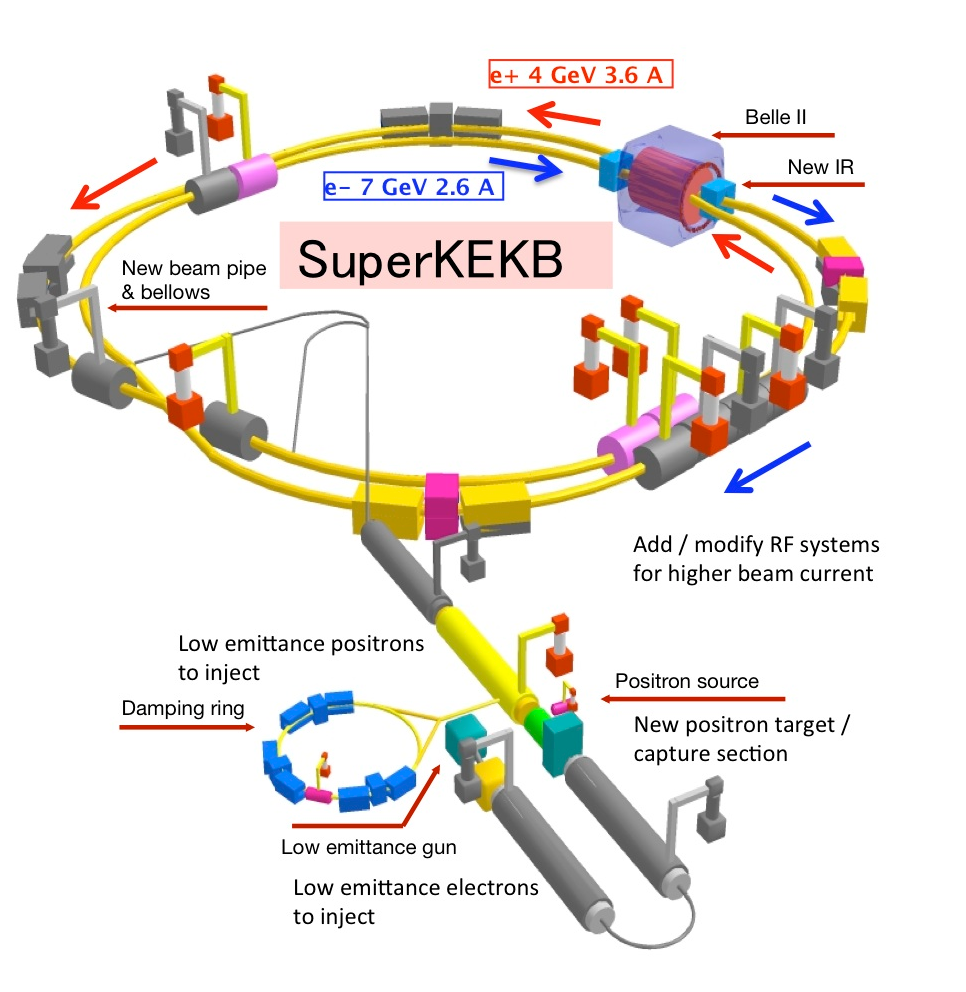
\includegraphics[width=0.7\textwidth]{SuperKEKB.png}
    \caption{Коллайдер SuperKEKB}
    \label{fig:galaxy}
\end{figure}
  Поскольку электронн-позитронные столкновения будут происходить с гораздо большей скоростью, необходимо было модернизировать детектор. Основные требования предъявляемые к детектору: 
\begin{itemize}
  \item Отличное разрешение вершин ($\approx$ 50 мкм)
  \item Очень высокая эффективность восстановления заряженных частиц с импульсами до нескольких сотен МэВ/с, и улучшенная эффективность для заряженных частиц с импульсами до 50 МэВ/с
  \item Очень хорошее разрешение импульса во всем кинематическом диапазоне эксперимента, т.е. до $\approx$ 8 ГэВ/с
  \item Точные измерения энергии и направления фотонов от нескольких десятков МэВ до $\approx$ 8 ГэВ и эффективное обнаружение с 30 МэВ и выше
  \item Высокоэффективная система идентификации частиц для разделения пионов, каонов, протонов и электронов и мюонов во всем кинематическом диапазоне эксперимента
  \item Полный охват телесного угла
  \item Быстрая и эффективная триггерная система, а также система сбора данных, способная хранить большое количество данных.
\end{itemize} \par
  Система сбора данных была перепроектирована с использованием оптических волокон. Электроника триггера была заменена новой системой. Был добавлен пиксельный детектор, обеспечивающий лучшее разрешение для отслеживания частиц, а новый кремниевый вершинный детектор будет покрывать больший телесный угол. Также были построены Центральная дрейфовая камера, времяпролетные счетчики и аэрогелевые черенковские счетчики. Детектор Belle II состоит из следующих подсистем:
\begin{itemize}
  \item Вершинный детектор (VXD) и пиксельный детектор (PXD), предназначенные для регистрации положения вершин распада частиц
  \item Центральная дрейфовая камера (CDC), которая предназначена для регистрации траектории частиц, импульсов и удельного энерговыделения заряженных частиц
  \item Время-проекционные счетчики (TOP) и аэрогелевые черенсковские счетчики (ARICH), служащие для определения заряженных частиц
  \item Электромагнитный калориметр (ECL), служит для регистрации фотонов и электронов, а также определения их энергий
  \item Детектор $K_{L}$ - мезонов и мюонов (KLM)
\end{itemize}
\begin{figure}[htp]
  \centering
  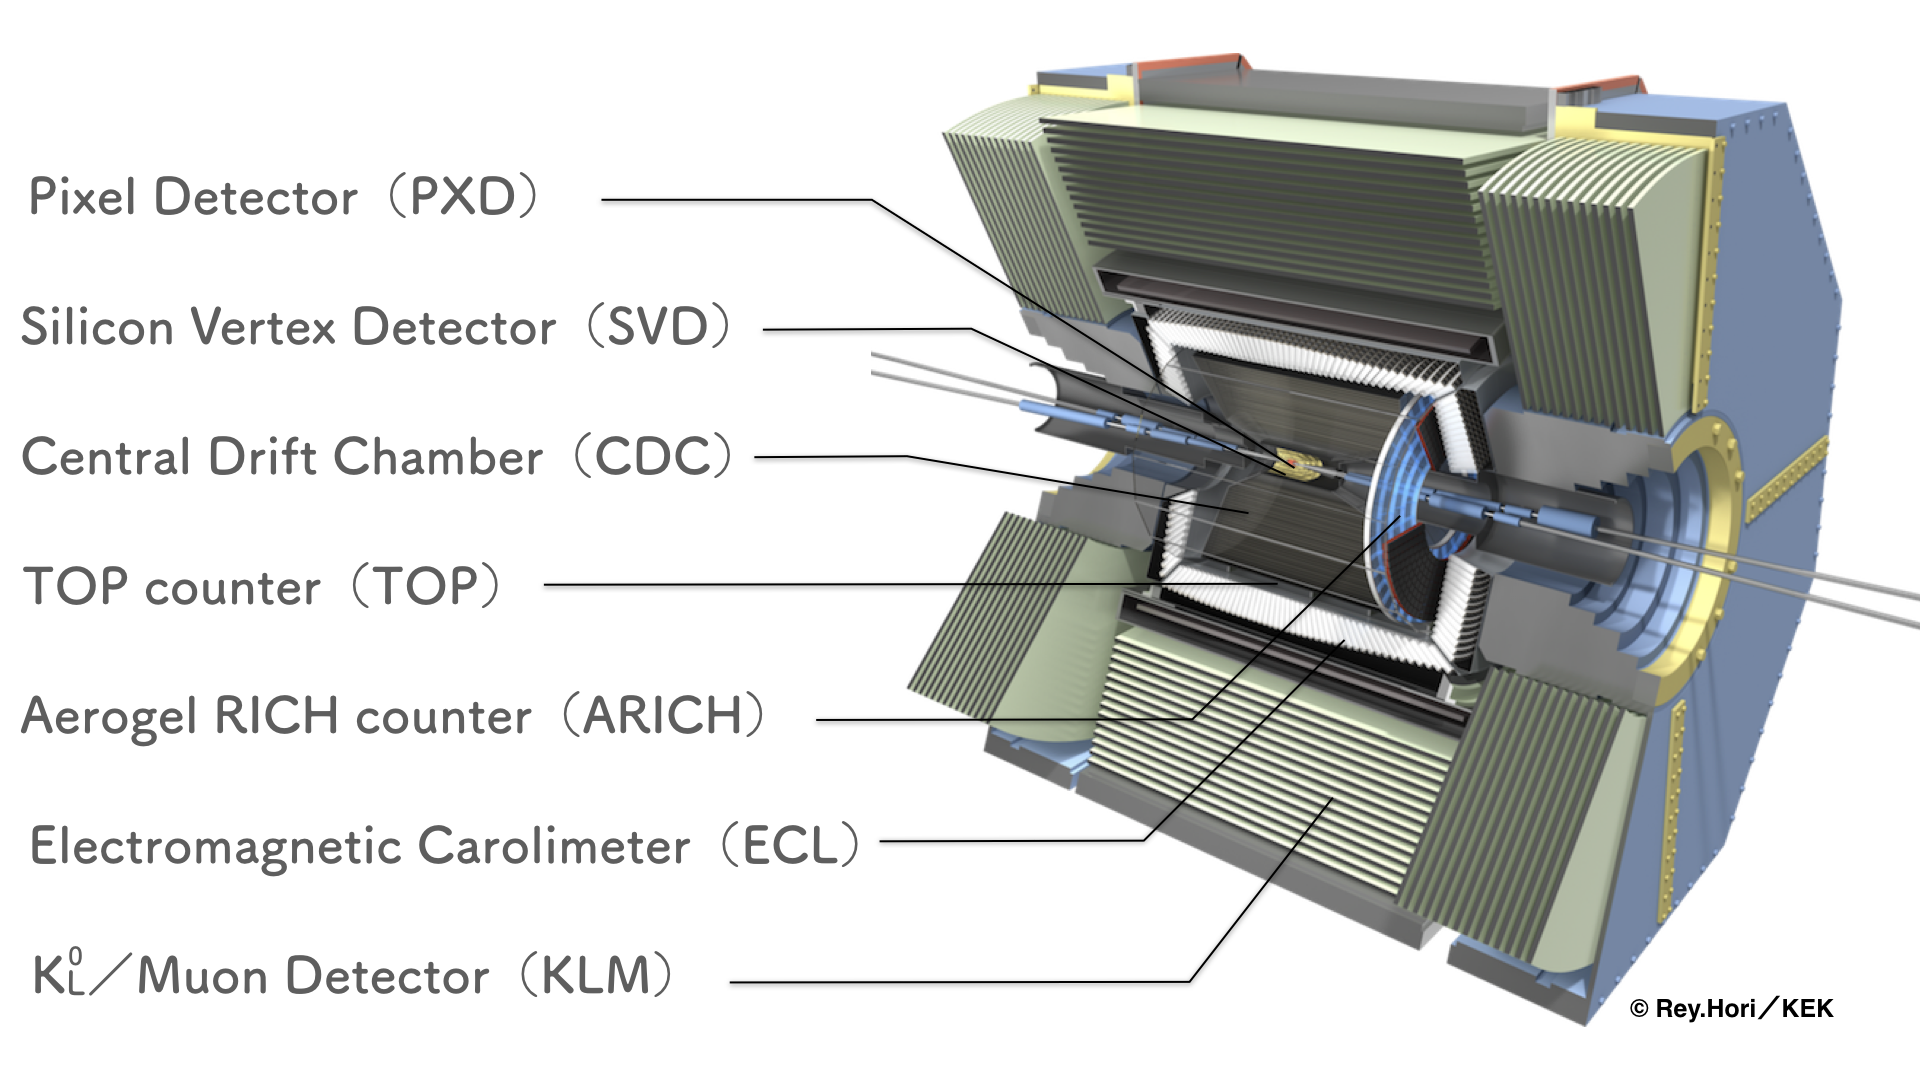
\includegraphics[width=\textwidth]{BelleII_detector.png}
  \caption{Детектор Belle II}
  \label{fig:galaxy}
\end{figure}
